%Code by GVV Sharma
%December 6, 2019
%released under GNU GPL
%Drawing a right angled triangle

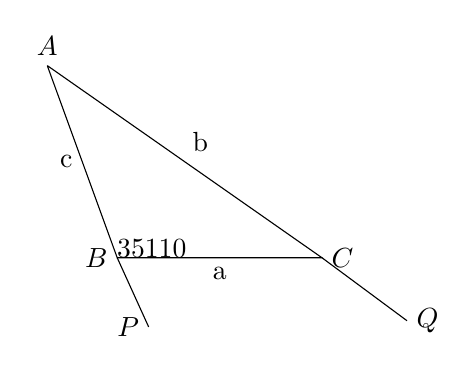
\begin{tikzpicture}[scale=0.4]

%Triangle sides
\def\a{6.5}
\def\c{6.5}
\def\b{10.64}

%Marking coordiantes
\coordinate [label=above:$A$] (A) at (-2.22,6.10);
\coordinate [label=left:$B$] (B) at (0,0);
\coordinate [label=right:$C$] (C) at (6.5,0);
\coordinate [label=left:$P$] (P) at (1,-2.2);
\coordinate [label=right:$Q$] (Q) at (9.2,-2);

%Drawing triangle ABC
\draw (A) -- node[left] {$\textrm{c}$} (B) -- node[below] {$\textrm{a}$} (C) -- node[above,,xshift=2mm] {$\textrm{b}$} (A);\draw (B)--(P);
\draw (C)--(Q);
%Drawing and marking angles
\tkzMarkAngle[arc=l,size=1,color=black](A,C,B)
\tkzLabelAngle[pos=1.5](A,C,B){\rotatebox{360}{$35$}}

\tkzMarkAngle[fill=white!40,size=0.5cm,mark=](C,B,A)
\tkzLabelAngle[pos=1](C,B,A){\rotatebox{-360}{$110$}}

\end{tikzpicture}

